%
% variation.tex
%
% (c) 2024 Prof Dr Andreas Müller
%
\begin{figure}
\centering
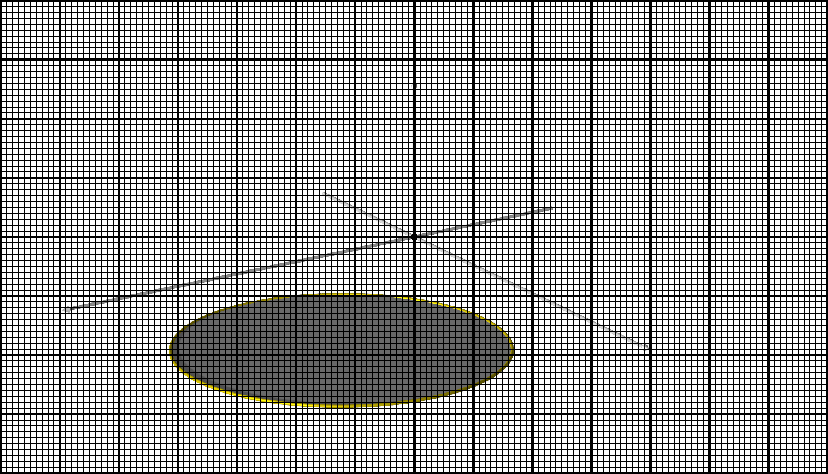
\includegraphics{chapters/040-felder/images/variation.pdf}
\caption{Variation einer Funktion von zwei Variablen.
Links die Funktion als Graph $z=\varphi(x,y)$, rechts die Variation
als Graphi $z=\varphi(x,y) + \varepsilon\eta(x,y)$ für verschiedene
Werte von $\varepsilon$.
\label{buch:felder:ostrogradski:fig:variation}}
\end{figure}
